\subsection{Структуры данных}

Для реализации программы требуется реализовать следующие структуры данных:

\begin{itemize}
    \item Граф, включая:
    \begin{itemize}
        \item Ключ вершины.
        \item Вершина графа.
        \item Ребро графа. 
    \end{itemize}
    \item Хранилище.
\end{itemize}

В таблице \ref{project-tbl:key} представлена структура ключа вершины. Ключ вершины должен быть произвольным, чтобы не привязываться к определённым вариантам ключей в реализации.
\begin{table}[h]
\centering
\caption{Структура данных ключа вершины.}
\begin{tabular}{|p{4cm}|p{4cm}|p{6cm}|}
\hline
Поле & Тип & Описание \\ 
\hline
key\_value & Произвольный & Значение ключа вершины \\
\hline
\end{tabular}
\label{project-tbl:key}
\end{table}

В таблице \ref{project-tbl:vertex} представлена структура вершины. Вершина имеет определяющий её ключ, бинарный массив с абсолютно произвольным набором данных параметров вершины, а также, для простоты рассылки и хранения, индексируемый список исходящих рёбер. Стоит отметить, что таким образом хранить рёбра неэффективно и не советуется, но для тестирования алгоритмов было решено прибегнуть к такому примитивному решению во имя простоты.

\begin{table}[h]
\centering
\caption{Структура данных вершины.}
\begin{tabular}{|p{4cm}|p{4cm}|p{6cm}|}
\hline
Поле & Тип & Описание \\ 
\hline
key & Ключ вершины & Ключ вершины \\ 
\hline
parameters & бинарный массив & Набор произвольных параметров вершины \\ 
\hline
edges & Индексируемый список рёбер & Список смежных рёбер \\ 
\hline
\end{tabular}
\label{project-tbl:vertex}
\end{table}

В таблице \ref{project-tbl:edge} представлена структура ребра. Ребро имеет запросный вес для структурной оптимизации на основе запросов,бинарный массив с абсолютно произвольным набором данных параметров ребра, включая осмысленный вес ребра в контексте хранимых данных, значение направленности ребра, а также ключи вершин, которые соединяет ребро.

\begin{table}[h]
\centering
\caption{Структура данных ребра}
\begin{tabular}{|p{4cm}|p{4cm}|p{6cm}|}
\hline
Поле & Тип & Описание \\ 
\hline
weight & Число & Запросный вес ребра \\ 
\hline
directional & 1/0 & Признак ориентированности ребра \\ 
\hline
parameters & бинарный массив & Набор произвольных параметров ребра \\ 
\hline
from & Ключ вершины & Начальная вершина \\ 
\hline
to & Ключ вершины & Конечная вершина \\
\hline
\end{tabular}
\label{project-tbl:edge}
\end{table}

Хранилище должно содержать информацию обо всех рёбрах внутри хранилища, а также рёбра, "исходящие" из него, для получения граничных вершин. Для этого была разработана древовидная структура данных состоящая из вложенных индексированных списков, названная "хранилище ветвей" и представленная на рисунке \ref{project-fig:external_edges}.

\begin{figure}[h]
    \centering
    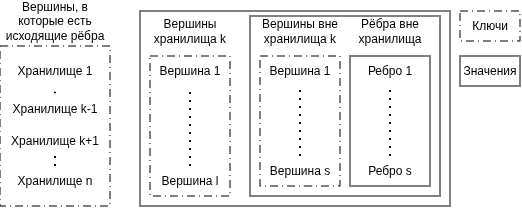
\includegraphics[width=\textwidth]{extras/contruction_part/external_edges.png}
    \caption{Схема "хранилища ветвей".}
    \label{project-fig:external_edges}
\end{figure}

Таблица \ref{project-tbl:storage} сожержит структуру данных хранилища. В хранилище содержатся вершины с внутренними рёбрами, хранилище ветвей, а также указательна шину для возможности общения с мастером и другими хранилищами.

\begin{table}[h]
\centering
\caption{Структура данных хранилища}
\begin{tabular}{|p{4cm}|p{4cm}|p{6cm}|}
\hline
Поле & Тип & Описание \\ 
\hline
id & Число & id хранилища \\ 
\hline
nodes & индексированный список вершин & вершины хранилища \\ 
\hline
external\_edges & хранилище ветвей & ребра, выходящие из хранилища \\ 
\hline
bus & указатель & указатель на шину для рассылок \\ 
\hline
\end{tabular}
\label{project-tbl:storage}
\end{table}